
%(BEGIN_QUESTION)
% Copyright 2010, Tony R. Kuphaldt, released under the Creative Commons Attribution License (v 1.0)
% This means you may do almost anything with this work of mine, so long as you give me proper credit

Anta at et bryggeri ønsker å installere en kapasitiv nivåprobe for å måle høyden av malt (delvis spirte byggkorn) i en lagringssilo:

$$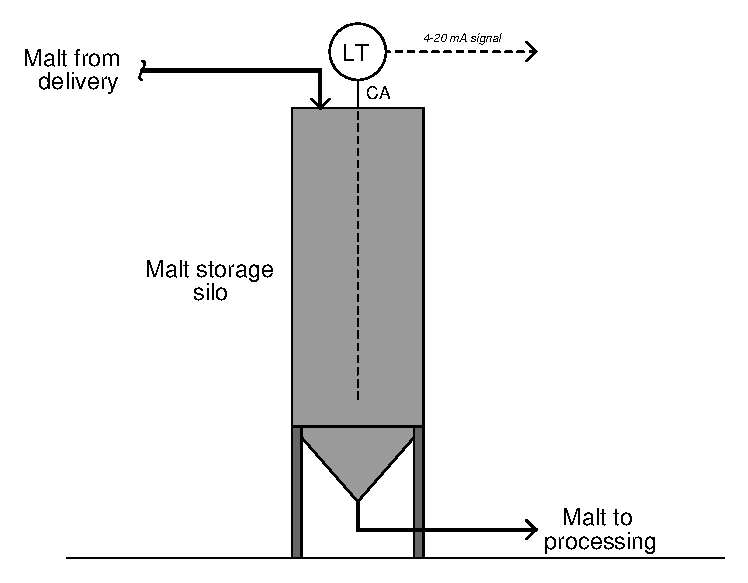
\includegraphics[width=15.5cm]{i00318x01.eps}$$

Dessverre gir det kapasitive nivåinstrumentet ikke stabile målinger av maltnivå, på grunn av variasjoner i maltens fuktinnhold fra leveranse til leveranse.  Våt malt har høyere bulk-permittivitet enn tørr malt, noe som gjør at nivåtransmitteren viser ulikt ved samme faktiske maltnivå i siloen.

\vskip 10pt

Driftslederen spør deg om en løsning på problemet.  Hva anbefaler du?

\vskip 20pt \vbox{\hrule \hbox{\strut \vrule{} {\bf Forslag til sokratisk diskusjon} \vrule} \hrule}

\begin{itemize}
\item{} Når malten er våtere, men faktisk nivå er uendret, vil LT vise høyere eller lavere nivå?  Forklar hvorfor.
\item{} Finnes det måter å få et kapasitivt instrument til å fungere bedre i denne applikasjonen?
\item{} For alternative teknologier du foreslår: angi hvordan hver av dem også kan få problemer ved måling av høyden på malt byggkorn i siloen.
\end{itemize}

\underbar{file i00318}
%(END_QUESTION)





%(BEGIN_ANSWER)


%(END_ANSWER)





%(BEGIN_NOTES)

Mulige alternativer til kapasitans-transmitter inkluderer:

\begin{itemize}
\item{} Vektmåling (forutsatt at fuktvariasjon ikke påvirker malttetthet for mye)
\item{} Guidet bølgeradar (forutsatt høy nok permittivitet for tydelig ekko)
\item{} Flottør på tilbaketrekkbart bånd
\item{} Ultralyd (forutsatt at rasvinkel ikke sprer lydbølger for mye)
\end{itemize}

%INDEX% Measurement, level: capacitance
%INDEX% Measurement, level: radar
%INDEX% Process: brewery malt storage tank level

%(END_NOTES)
